\documentclass[12pt]{article}
\usepackage[a4paper]{geometry}
\usepackage{fullpage}
\usepackage[T1]{fontenc}
\usepackage[utf8]{inputenc}
\usepackage{graphicx}
\usepackage{mathpazo}
\pagenumbering{gobble}
\usepackage{siunitx}
\sisetup{output-decimal-marker = {,}}
\usepackage{amsmath}
\usepackage{esdiff}
\usepackage[spanish]{babel}
\newcommand{\laplace}[1]{\mathbf{#1}(\mathbf{s})}
\newcommand{\slp}{\mathbf{s}}

\begin{document}

\title{\textsc{Teoría de Circuitos III}\\Prueba BT3}

\date{22 de noviembre de  2018\\\small{Los resultados se publicarán el día 2 de diciembre.\\La revisión del examen se realizará el 3 de diciembre de 11:30 a 14:30.}}

\maketitle

La figura representa un circuito que comienza un régimen transitorio a partir de unas condiciones iniciales definidas por $v_{c}(0^-) = \SI{1}{\volt}$ y $i_L(0^-) = \SI{0}{\ampere}$. En este ejercicio se analizará el régimen transitorio del circuito con variables de estado, empleando como tales $v_{c}(t)$ y  $i_L(t)$.

\begin{enumerate}

\item (\textbf{0.5p}) Determina los valores en régimen permanente de las variables.
  
\item  (\textbf{2p}) Dibuja el grafo del circuito, y elige un árbol propio. En este grafo deben quedar indicadas las variables con polaridad y sentido, según corresponda.
  
\item  (\textbf{2.5p}) Determina las ecuaciones necesarias para cada variable de estado, obteniendo la ecuación de estado en forma matricial. Es necesario indicar claramente las expresiones de las variables adicionales que sean necesarias.
  
\item  (\textbf{2.5p}) Determina las expresiones de las variables de estado en el dominio de Laplace.
  
\item (\textbf{0.5p}) Determina los polos del sistema y, sin resolver la ecuación de estado, estima de forma justificada el tipo de transitorio presente en el circuito.
  
\item  (\textbf{2p}) Calcula las expresiones en el dominio del tiempo de las variables de estado. Indica de forma expresa el cumplimiento de las condiciones iniciales y los valores en el régimen permanente.
  
\end{enumerate}


\begin{minipage}{0.3\textwidth}
Datos:
\begin{align*}
  E_g &= \SI{1}{\volt}\\
  R_1 &= \SI{2/5}{\ohm}\\
  R_2 &= \SI{2/3}{\ohm}\\
  L &= \SI{4/3}{\henry}\\
  C &= \SI{1}{\farad}
\end{align*}
\end{minipage}
\begin{minipage}{0.7\textwidth}
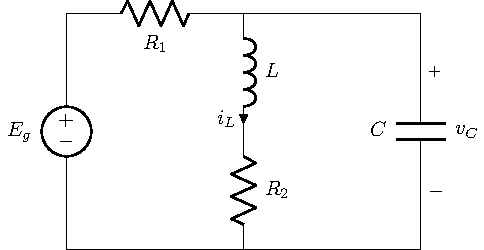
\includegraphics{figs/E3_circuito.pdf}
\end{minipage}

\section*{Solución}

\begin{enumerate}
\item Régimen permanente

  Sustituyendo los equivalentes de bobina y condensador en régimen permanente obtenemos:

  \begin{align*}
    u_c(\infty) &= E_g \cdot \frac{R_2}{R_1 + R_2} = \SI{5/8}{\volt} = \SI{0.625}{\volt}\\
    i_L(\infty) &= \frac{E_g}{R_1 + R_2} = \SI{15/16}{\ampere} = \SI{0.9375}{\ampere}
  \end{align*}
  
\item Grafo

  La figura representa el grafo del circuito, en el que se ha resaltado el árbol propio, y se han indicado las flechas de las variables de estado y las variables auxiliares.

  \begin{center}
    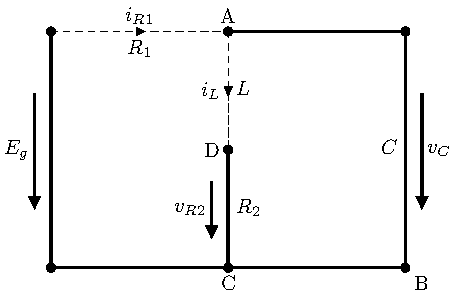
\includegraphics{figs/E3_grafo.pdf}
  \end{center}
  
\item Ecuación de estado

  Para obtener la ecuación de la variable de estado $v_c(t)$ utilizamos la LKC en el grupo del corte básico A:

  \[
    i_{R1} = i_L + C\diff{u_c}{t}
  \]

  Para obtener la ecuación de la variable de estado $i_L(t)$ utilizamos la LKV en el lazo básico ABCDA:

  \[
    u_c - u_{R2} - L\diff{i_L}{t} = 0
  \]

  Las variables auxiliares $i_{R1}$ y $u_{R2}$ quedan definidas con las siguientes ecuaciones:

  \begin{align*}
    i_{R1} &= \frac{E_g - u_c}{R_1}\\
    u_{R2} &= i_L \cdot R_2
  \end{align*}

  Reescribiendo estas ecuaciones en forma matricial obtenemos:

  \[
    \left[
      \begin{array}{c}
        \dot{U}_c\\
        \dot{I}_L
      \end{array}
    \right] =
    \left[
      \begin{array}{cc}
        -1/R_1C & -1/C\\
        1/L & -R_2/L
      \end{array}
    \right] \cdot
    \left[
      \begin{array}{c}
        U_c\\
        I_L
      \end{array}
    \right] +
    \left[
      \begin{array}{c}
        1/R_1C\\
        0
      \end{array}
    \right] \cdot E_g
  \]


Sustituyendo valores tenemos:

  \[
    \left[
      \begin{array}{c}
        \dot{U}_C\\
        \dot{I}_L
      \end{array}
    \right] =
    \left[
      \begin{array}{cc}
        -2.5 & -1\\
        0.75 & -0.5
      \end{array}
    \right] \cdot
    \left[
      \begin{array}{c}
        U_c\\
        I_L
      \end{array}
    \right] +
    \left[
      \begin{array}{c}
        2.5\\
        0
      \end{array}
    \right] \cdot 1
  \]


\item Ecuación de estado con Laplace

  La expresión general es:
  \[
    \laplace{X} = \left(\slp \mathbf{I} - \mathbf{A} \right)^{-1} \mathbf{x}(0^-) + \left(\slp \mathbf{I} - \mathbf{A} \right)^{-1} \mathbf{B}\laplace{U}
  \]
  que, sustituyendo lo obtenido en el apartado anterior, nos lleva a:

    \[
    \left[
      \begin{array}{c}
        \laplace{U_c}\\
        \laplace{I_L}
      \end{array}
    \right] =
    \left(\slp \mathbf{I} - \mathbf{A} \right)^{-1} \cdot
    \left[
      \begin{array}{c}
        1\\
        0
      \end{array}
    \right] +
    \left(\slp \mathbf{I} - \mathbf{A} \right)^{-1} \cdot
    \left[
      \begin{array}{c}
        2.5\\
        0
      \end{array}
    \right] \cdot 1/\slp
  \]
siendo
\[
  \left(\slp \mathbf{I} - \mathbf{A} \right) = 
  \left[
    \begin{array}{cc}
    \slp + 2.5 &  1\\
    -0.75 & \slp +0.5
  \end{array}
\right]
\]


El determinante de esta matriz es:

\[
  \det{\left(\slp \mathbf{I} - \mathbf{A} \right)} = (\slp + 1)(\slp + 2)
\]

La matriz inversa es:

\[
  \left(\slp \mathbf{I} - \mathbf{A} \right)^{-1} = 
  \frac{1}{(\slp + 1)(\slp +2)} \cdot \left[
     \begin{array}{cc}
       \slp + 0.5 &  -1\\
       0.75 & \slp + 2.5
     \end{array}
   \right]
\]

Por tanto,

\begin{align*}
  \laplace{U_C} &= \frac{\slp^2 + 3\slp + 1.25}{\slp(\slp + 1)(\slp +2)}\\
  \laplace{I_L} &= \frac{0.75\slp + 1.875}{\slp(\slp + 1)(\slp +2)}
\end{align*}

\item Los polos de este circuito están situados en $\slp = -1$ y $\slp = -2$. Al tratarse de dos polos reales y distintos, podemos afirmar que el transitorio presente en el circuito es sobreamortiguado (dos exponenciales decrecientes).


\item Resolución de la ecuación de estado

Aplicando desarrollo en fracciones parciales para cada variable obtenemos:

\begin{align*}
  u_C(t) &= 0.625 + 0.75 e^{-t} - 0.375 e^{-2t}\\
  i_L(t) &=  0.9375 - 1.125 e^{-t} + 0.1875 e^{-2t}\\
\end{align*}

Se puede comprobar que estas expresiones cumplen las condiciones iniciales y los valores en régimen permanente. Además, tal y como se indicó anteriormente, se trata de un transitorio sobreamortiguado, con la superposición de dos exponenciales decrecientes cuyos exponentes coinciden con los polos detectados.
\end{enumerate}
\end{document}

% Local Variables:
% ispell-local-dictionary: "castellano"
% End:

